\chapter{Theory}


\section{Wave Theory}

Simple Wave Theory

\section{Energy Spectra}

\subsection{Phillips Spectrum}
\subsection{Mobley Spectrum}
\subsection{SWAP}
\subsection{JONSWAP}


Energy Spectrum

$\int x(t) dt$

$k=\frac{\pi}{\mathbf y}$

\begin{equation}\label{eq:test} x = y \end{equation}

We can give an equation a label so that we can refer to it later.
\begin{equation}
\label{eq:ising}
E = -J \sum_{i=1}^N s_i s_{i+1} ,
\end{equation}
Equation~\eqref{eq:ising} expresses the energy of a configuration
of spins in the Ising model.

\section{The Rendering Pipeline}
The rendering pipeline constitutes the core of real-time graphics. It's task
consists in generating, or rendering, a two-dimensional output image given a
virtual camera, scene geometry, materials and
lightsources\cite{book:akenine-rtr}. As shown in Figure~\ref{fig:RAGR} the
rendering pipeline can be divided into three conceptual stages:
\begin{itemize}
 \item The \textit{application stage} holds all necessary information to break
down the scene geometry into smaller chunks which actually are passed on to the
geometry stage.
 \item The \textit{geometry stage} transforms the input geometry to a
two-dimensional output coordinate system.
 \item The \textit{rasterizer stage} fills the primitives output by the
geometry stage with color.
\end{itemize}

\begin{figure}
\begin{center}
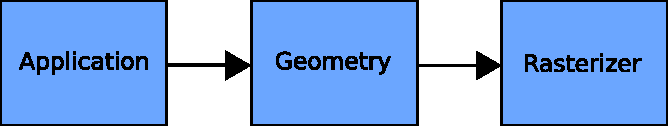
\includegraphics[scale=0.8]{Images/Rendering-Pipeline-AGR.pdf}
\caption{The three stages of the rendering pipeline.}
\label{fig:RAGR}
\end{center}
\end{figure}

\subsection{Application Stage}
The application stage implements the whole program logic, user input and
consequently the application's internal state is managed by the application
stage. It's main responsibility lies in deciding what is actually to be
visualised and therefore feeding the geometry stage with the selected data.
The actual implementation of the application stage is entirely dependent on
it's task. 
A common task which resides in the application stage is \textit{collision
detection and response}: to detect if two objects collide and update their
internal state accordingly. Nowadays this is often done by a physics library
tailored to this task, such as NVIDIA PhysX\cite{misc:ageia-physx} and Havok
Physics\cite{misc:havok}. Those libraries are capable of complex physics
simulations, their collision detection and respinse capabilities are a mere,
but rather welcome, side effect.
Whereas the geometry and rasterizer stages are to be found on the graphics
hardware, the application stage is executed in software on the CPU side.
software stage, excempt hardware accelerated physics and sound
holds high level scene information
prepares data to be processed by geometry stage
collision detection
physics
visibility culling

\subsection{Geometry Stage}

model coordinates
model matrix
world coordinates
view matrix
view coordinates
projection matrix
clip coordinates, cube
clipping
perspective division
normalized device coordinates, unit cube
viewport transformation
window coordinates
\begin{figure}
\begin{center}
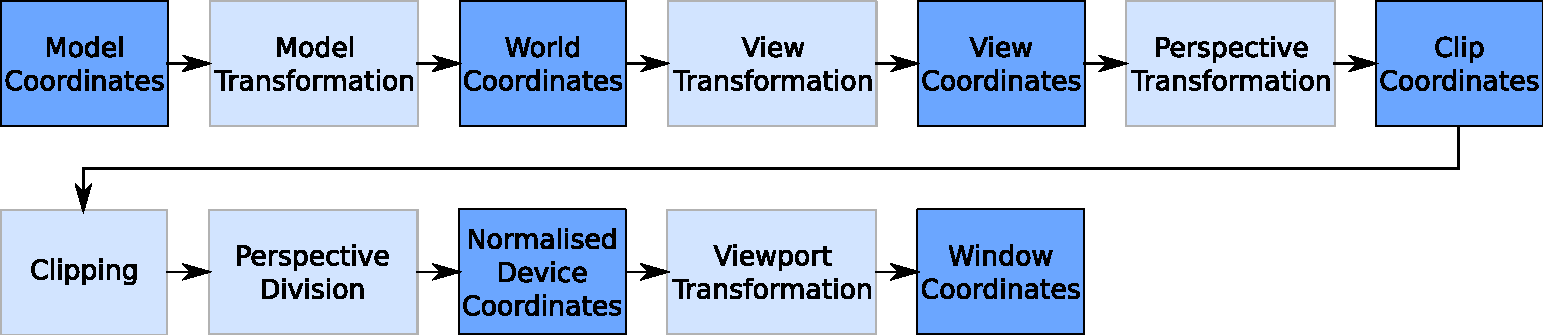
\includegraphics[scale=0.5]{Images/Geometry-Stage.pdf}
\caption{The Geometry stage.}
\label{fig:GeometryStage}
\end{center}
\end{figure}


\subsection{Rasterizer Stage}

triangle setup
scan conversion and interpolation
per fragment operations (texturing, ummadumshadern)
\begin{figure}
\begin{center}
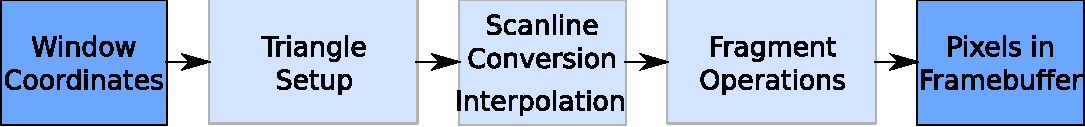
\includegraphics[scale=0.5]{Images/Rasterizer-Stage.pdf}
\caption{The Rasterizer stage.}
\label{fig:RasterizerStage}
\end{center}
\end{figure}

\section{The Projected Grid}

postprojection coordinates transformed to worldspace
grid on near and far plane, intersection with the y=0 plane
decouple projector from camera

\subsection{The Projector}
positioning
rotating
original is a hack, persistent grid mapping has a more stable approach
not optimal, because of "popping" at great distances
not so optimal distribution of the mesh resolution throughout worldspace
visual range issues
do some modifications to the mesh vertex distribution
reference to original paper from 2004 + persistent grid mapping

\section{Water optics}
BRAK

\section{Colour Management}

Explain color and gamma problem
linear vs nonlinear space

\subsection{gamma}
sRGB(gamma 2.2) support in hardware, convert from nonlinear space to linear
space do calculations on lighting and so on, back to srgb space
do tonemapping sRGB -> XYZ -> xyY -> modify Y -> XYZ -> sRGB

\subsection{device calibration}
short explanation of monitor calibration and so on
tools available


